\documentclass[11pt]{article}
\usepackage{minibox}
\usepackage[top=1in, bottom=1.25in, left=1.25in, right=1.25in]{geometry}
\newcommand{\tabitem}{~~\llap{\textbullet}~~}
\usepackage[parfill]{parskip}
\usepackage{enumerate}
\usepackage{amsmath}
\usepackage{amsthm}
\usepackage[shortlabels]{enumitem}
\usepackage{amssymb}
\usepackage{ bbold }
\usepackage{graphicx} %included to insert a graph
\usepackage{caption} %included to include a caption over the graph
\usepackage{booktabs} %needed for the table's toprule midrule and bottomrule sequences
\usepackage[section]{placeins} %to keep graphs and tables in the very section to which they belong 
\usepackage{pdflscape} %to include the landscape environment 
\usepackage[T1]{fontenc}
\usepackage{multirow}
\usepackage{verbatim}
\usepackage{subcaption}
\usepackage{pdfpages}
\usepackage{lscape}
%-----------------------------------------------------------------------------
\begin{document}
\begin{center}
\framebox[\linewidth]{ 
	\minibox[c]{
	\Large Econ 244 - Homework \#4 \\ \\
	}
}
\end{center}

\begin{enumerate}[1)]
	\item (CRE vs Fixed Effects)

	\begin{enumerate}[(a)]
	
		\item Prove that the LSDV estimator of this model is consistent for $\beta$:

		The LSDV estimator is given estimating
		\begin{align*}
		 	Y_{it} &= \sum_{j=1}^N \gamma_j D^j_{it} + \beta X_{it} + \epsilon_{it}
		\end{align*}

		By the Frisch-Waugh-Lovell theorem, the estimated coefficient $\beta$ is equivalent to regressing $\tilde{Y}_{it}$ on $\tilde{X}_{it}$, $\tilde{Y}_{it}$ and $\tilde{X}_{it}$ are the regressions of $Y$ and $X$ on the dummy variables. This is equivalent to demeaning the variables by individual $i$, so $\tilde{Y}_{it} = Y_{it} - \bar{Y}_i$ and $\tilde{X}_{it} = X_{it} - \bar{X}_i$. This is consistent for $\beta$ if $E[\tilde{\epsilon}_{it} \tilde{X}_{it}] = 0$:
		\begin{align*}
			E[\tilde{\epsilon}_{it} \tilde{X}_{it}] &= E[(\epsilon_{it} - \bar{\epsilon}_i) (X_{it} - \bar{X}_i)] \\
			&= E[(\epsilon_{it} - \bar{\epsilon}_i) (X_{it} - \bar{X}_i)]
		\end{align*}
		which holds if there is strict exogeneity of $\epsilon_{it}$, because $\bar{\epsilon}_i$ is a function of future and lag values of $\epsilon_{it}$ as well; that is, if $X_{it}$ is uncorrelated with not only $\epsilon_{it}$ but also future and lag values of $\epsilon_{it}$.

		\item Show that estimating $Y_{it} = \alpha_0 + \alpha_1 \bar{X}_i + \beta X_{it} + u_{it}$ yields the same estimate as the LSDV estimator:

		By using the F-W-L theorem, estimating the above is equivalent to estimating
		\begin{align*}
			Y_{it} - \bar{Y} &= \alpha_1 (\bar{X}_i - \bar{X}) + \beta (X_{it} - \bar{X}) + (u_{it} - \bar{u}) 
		\end{align*}
		That is, regressing the population-demeaned variables on each other without a constant. Applying F-W-L again, note that the annihilator matrix for $\bar{X}_i - \bar{X}$ is
		\begin{align*}
			M &= I - \frac{1}{T \sum_{j} (\bar{X}_j - \bar{X})^2} \begin{bmatrix} [(\bar{X}_{i} - \bar{X})(\bar{X}_{j} - \bar{X})] \end{bmatrix}
		\end{align*}
		that is, every element of the last term is $(X_{i} - \bar{X})(X_j - \bar{X})$. Applying the annihilator matrix to the LHS, the $i$th element of the LHS vector is
		\begin{align*}
			(M Y)_i &= Y_{it} - \bar{Y} - \frac{(\bar{X}_i - \bar{X}) \sum_{j,t} \left( \bar{X}_j - \bar{X} \right) \left( Y_{jt} - \bar{Y} \right)  }{T \sum_{j} (\bar{X}_j - \bar{X})^2} \\
			&= Y_{it} - \bar{Y} - \frac{(\bar{X}_i - \bar{X}) \sum_{j} \left( \bar{X}_j - \bar{X} \right) \sum_t \left( Y_{jt} - \bar{Y} \right)  }{T \sum_{j} (\bar{X}_j - \bar{X})^2} \\
			&= Y_{it} - \bar{Y} - \frac{(\bar{X}_i - \bar{X}) \sum_{j} \left( \bar{X}_j - \bar{X} \right) \left( \bar{Y}_j - \bar{Y} \right)  }{\sum_{j} (\bar{X}_j - \bar{X})^2} \\
			&= Y_{it} - \bar{Y} - \frac{(\bar{X}_i - \bar{X}) \sum_{j} \left( \bar{X}_j - \bar{X} \right) \left( [a_0 + a_1 \bar{X}_j + \beta \bar{X}_j + \bar{u}_j] - [a_0 + a_1 \bar{X} + \beta \bar{X} + \bar{u}] \right)  }{\sum_{j} (\bar{X}_j - \bar{X})^2} \\
			&= Y_{it} - \bar{Y} - \frac{(\bar{X}_i - \bar{X}) \sum_{j} \left( \bar{X}_j - \bar{X} \right) \left( (a_1 + \beta) (\bar{X}_j - \bar{X}) + \bar{u}_j - \bar{u} \right)  }{\sum_{j} (\bar{X}_j - \bar{X})^2} \\
			&= Y_{it} - \bar{Y} - (a_1 + \beta) (\bar{X}_i - \bar{X}) - \frac{(\bar{X}_i - \bar{X}) \sum_{j} \left( \bar{X}_j - \bar{X} \right) \left( \bar{u}_j - \bar{u} \right)  }{\sum_{j} (\bar{X}_j - \bar{X})^2} \\
			&= Y_{it} - \bar{Y}_i
		\end{align*}
		and similar algebra applied to regressing $X_{it} - \bar{X}$ on $\bar{X}_i- \bar{X}$ shows that the full regression is equivalent to regressing $Y_{it} - \bar{Y}_i$ on $X_{it} -\bar{X}_i$, which is the same as LSDV.

		\item Describe a procedure for testing for zero correlation between the person effects and $X_{it}$: one could regress $T_{it}$ on $\bar{X}_{it}$ and $X_{it}$, as before, and t-test the hypothesis that the coefficient on $\bar{X}_{it}$ is 0. If one rejects the hypothesis, then that is evidence for correlation between the person effects and $X_{it}$.

		\item Propose estimators for $Var(v_i)$ and $Var(\alpha_i)$:

		For $Var(v_i)$, an estimator is the saple variance, given by $\frac{1}{N-1} \sum_i (\hat{\alpha}_i - \hat{a}_0 - \hat{a}_1 \bar{X}_i)^2$, where $\hat{\alpha}$ is taken from the fixed-effects regression and $\alpha_0$ and $\alpha_1$ is taken from the regression from part (b). 

		For $Var(\alpha_i)$, since $\alpha_i = a_0 + a_1 \bar{X}_i + v_i$, the estimator for $\alpha_i$ is $Var(\bar{X}_i) + \hat{Var}(v_i)$.
	
	\end{enumerate}
	

	\item (Event Study)
	\begin{enumerate}[(a)]
		\item See do file.
		\item See do file and table \ref{q2b}. \\
		\begin{table}[htbp]\centering \scriptsize
\def\sym#1{\ifmmode^{#1}\else\(^{#1}\)\fi}
\caption{Question 2b and 2e \label{q2b}}
\begin{tabular}{l*{2}{c}}
\toprule
                    &\multicolumn{1}{c}{(1)}&\multicolumn{1}{c}{(2)}\\
                    &\multicolumn{1}{c}{Log Arrests}&\multicolumn{1}{c}{Log Arrests}\\
\midrule
0                   &     -0.0724*  &     -0.0447   \\
                    &   (0.04097)   &   (0.03410)   \\
\addlinespace
1                   &      -0.153** &     -0.0994*  \\
                    &   (0.06718)   &   (0.05405)   \\
\addlinespace
2                   &      -0.179*  &      -0.103   \\
                    &   (0.09928)   &   (0.08530)   \\
\addlinespace
3                   &      -0.196*  &     -0.0969   \\
                    &   (0.11195)   &   (0.09814)   \\
\addlinespace
4                   &      -0.216   &     -0.0984   \\
                    &   (0.13955)   &   (0.13022)   \\
\addlinespace
5                   &      -0.254   &      -0.127   \\
                    &   (0.15976)   &   (0.15272)   \\
\addlinespace
6                   &      -0.337*  &      -0.188   \\
                    &   (0.18844)   &   (0.18051)   \\
\addlinespace
7                   &      -0.381*  &      -0.225   \\
                    &   (0.21022)   &   (0.21005)   \\
\addlinespace
8                   &      -0.357*  &      -0.206   \\
                    &   (0.21014)   &   (0.21727)   \\
\addlinespace
9                   &      -0.463*  &      -0.293   \\
                    &   (0.25040)   &   (0.25997)   \\
\addlinespace
10                  &      -0.561*  &      -0.423   \\
                    &   (0.31938)   &   (0.37817)   \\
\addlinespace
-2                  &     0.00306   &     -0.0266   \\
                    &   (0.04029)   &   (0.03919)   \\
\addlinespace
-3                  &      0.0505   &     -0.0118   \\
                    &   (0.06806)   &   (0.06462)   \\
\addlinespace
-4                  &      0.0744   &     -0.0217   \\
                    &   (0.09482)   &   (0.07838)   \\
\addlinespace
-5                  &      0.0634   &     -0.0682   \\
                    &   (0.12321)   &   (0.09156)   \\
\addlinespace
-6                  &      0.0756   &      -0.116   \\
                    &   (0.15743)   &   (0.11055)   \\
\addlinespace
-7                  &      0.0681   &      -0.163   \\
                    &   (0.19197)   &   (0.13063)   \\
\addlinespace
-8                  &      0.0822   &      -0.174   \\
                    &   (0.22642)   &   (0.15078)   \\
\addlinespace
-9                  &      0.0243   &      -0.277   \\
                    &   (0.26328)   &   (0.17508)   \\
\addlinespace
-10                 &      0.0862   &      -0.342   \\
                    &   (0.33427)   &   (0.20880)   \\
\addlinespace
Constant            &       6.545***&       6.556***\\
                    &   (0.26179)   &   (0.10881)   \\
\midrule
Year Fixed Effects & X & X \\
City Fixed Effects & X & X \\
City-Specific Time Trend & & X \\
\midrule
\(R^{2}\)           &       0.804   &       0.870   \\
Observations        &        1297   &        1297   \\
\bottomrule
\multicolumn{3}{l}{\footnotesize Standard errors in parentheses}\\
\multicolumn{3}{l}{\footnotesize * p<0.10, ** p<0.05, *** p<0.01}\\
\end{tabular}
\end{table}

		\item  It appears arrests go down in the years following the policy relative just before the curfew was put in place. In the years prior to the policy, arrest rates were fairly flat. However, the estimates are fairly imprecise outside of a couple year band around the policy. Note that data from 10 years before the policy and 10 years after were binned into the -10 and 10 dummies.\\
		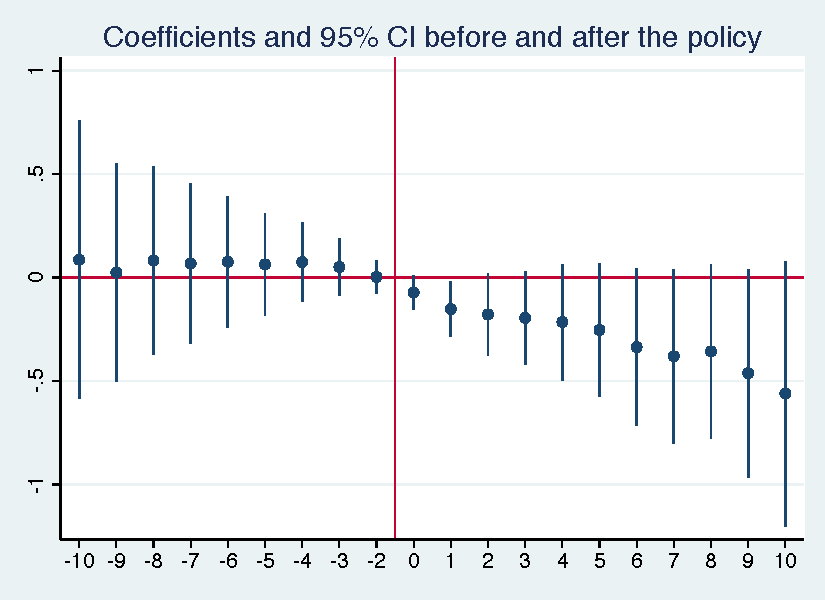
\includegraphics[scale=.8]{input/coef_plot_10year.pdf}
		\item We can restrict our analysis to just look 5 years before and after the policy or 12 years before and after. We can see a slight change in the coefficients but the general pattern is similar--that arrest rates were fairly flat beforehand and decreased in the years after the policy.\\
			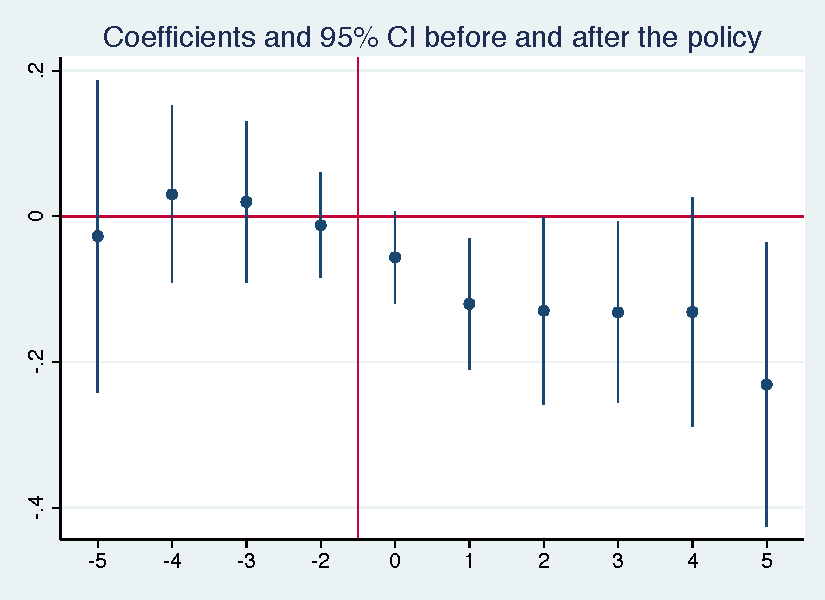
\includegraphics[scale=.8]{input/coef_plot_5year.pdf} \\
			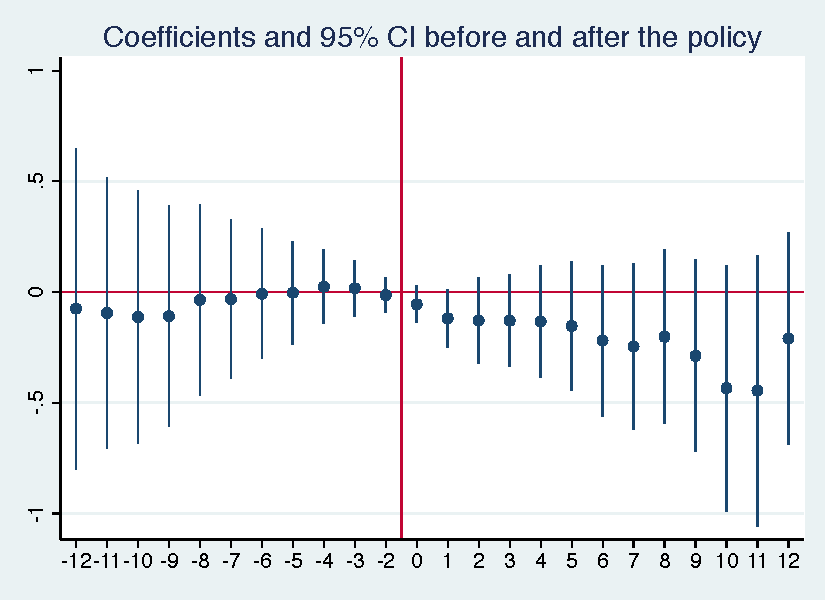
\includegraphics[scale=.8]{input/coef_plot_12year.pdf}
		
		\item When we add a linear city-specific trend, we get a slightly different story from the data. It appears that arrests were slightly increasing prior to the policy change and then decreased afterwards. Perhaps explaining the impetus for the policy change. \\
			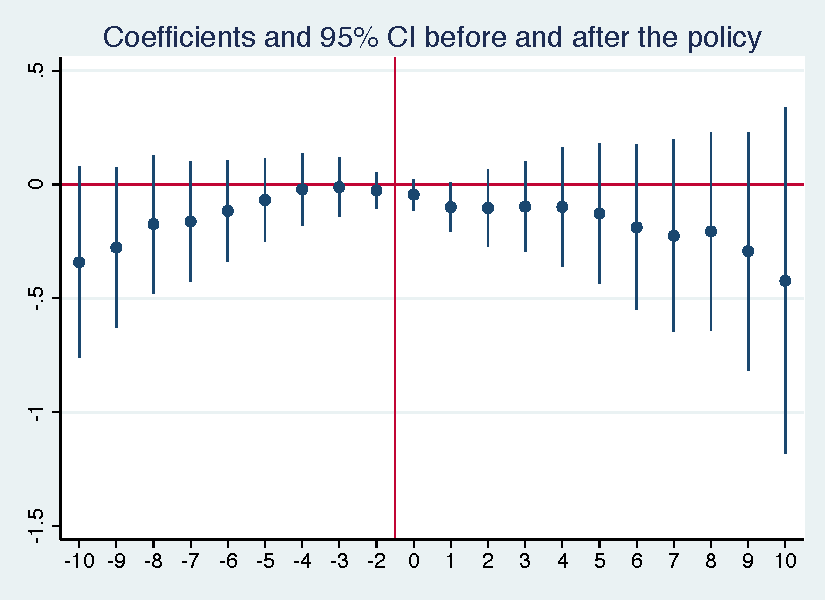
\includegraphics[scale=.8]{input/coef_plot_10year_trend.pdf}
	\end{enumerate}
	\item (Dynamic Panel)
	\item (CRE Event Study)
	\begin{enumerate}[(a)]
		\item See do file.
		\item Estimating the model with ``mvreg''. See Table~\ref{Unconstrained}
		\item To ease notation, let $H \equiv \{85,87,88,89,90\}$ be the set of event dates.

		First, observe that we can write $\pi_{k,t}$ as including the dynamic causal effects as well as the endogenous component. That is, we can write:
		\[\pi_{k,t} = \delta_{t-k}\mathbf{1}(t \geq k) + \eta_k \]

		As is stated in the original problem, this directly implies the first set of linear restrictions:
		\[\pi_{k,t} = \pi_{k,t'} \mbox{ } \forall (t,t') < k\]

		Next, observe that for all $h$ such that $k, k' \in H$ and for all $t$ and $s$, we have
		\begin{align*}
			\pi_{k',k'+t} - \pi_{k,k+t} & = \eta_{k'} - \eta_{k} \\
			& = \pi_{k',k'+s} - \pi_{k,k+s}
		\end{align*}

		Similarly, we also have for $k,k'\in H$ and $t$ and $s$:
		\begin{align*}
			\pi_{k,k+t+s} - \pi_{k,k+t} & = \delta_{t+s} - \delta_{t} \\
            & = \pi_{k',k'+t+s} - \pi_{k',k'+t}
		\end{align*}

		The final set of constraints identify each $\delta_k$ separately. For all $k,k' \in H$, for all $t,t'$ and all $s$:
		\begin{align*}
			\pi_{k,k+s} - \pi_{k,k-t} & = \delta_{s} \\
			& = \pi_{k',k'+s} - \pi_{k',k'-t'}
		\end{align*}

		\item Using the \textit{constraint} function in Stata along with \textit{sureg}, we can estimate the model under the constraints specified in part (c), of which only 26 were needed to span the entire set.\footnote{Note: I did this in a rather brute force manner. Rather than figuring out analytically the minimal set of constraints necessary to span the entire space of constraints, I looped over each of these constraint sets and allowed Stata to remove those that were redundant.} These estimates are given in the Table~\ref{Constraint_Est}

		Using \textit{lincom} we can identify each $\delta_k$ as the difference $\pi_{85,85+k}-\pi_{85,84}$ which removes the endogenous component appearing in both terms, leaving only the $k^{th}$ dynamic term. See Table~\ref{Lincoms}
		
	\end{enumerate}
\end{enumerate}

\appendix

\begin{table}
	\caption{Estimating the Model with \textit{mvreg}}
	\label{Unconstrained}
	\centering
	{
\def\sym#1{\ifmmode^{#1}\else\(^{#1}\)\fi}
\begin{tabular}{l*{7}{c}}
\hline\hline
            &\multicolumn{7}{c}{Log of Arrests Made in}                                                                     \\
            &        1984   &        1985   &        1986   &        1987   &        1988   &        1989   &        1990   \\
            &        b/se   &        b/se   &        b/se   &        b/se   &        b/se   &        b/se   &        b/se   \\
\hline
Enacted in 1985&       -0.50   &       -0.76   &       -0.71   &       -0.60   &       -0.59   &       -0.65   &       -0.85   \\
            &      (0.66)   &      (0.64)   &      (0.72)   &      (0.76)   &      (0.72)   &      (0.71)   &      (0.68)   \\
Enacted in 1987&        0.70   &        0.49   &        0.47   &        0.20   &        0.03   &        0.06   &        0.03   \\
            &      (0.47)   &      (0.46)   &      (0.52)   &      (0.54)   &      (0.52)   &      (0.51)   &      (0.49)   \\
Enacted in 1988&        1.01** &        0.92** &        1.01*  &        1.08*  &        1.18** &        1.16** &        1.18** \\
            &      (0.47)   &      (0.46)   &      (0.52)   &      (0.54)   &      (0.52)   &      (0.51)   &      (0.49)   \\
Enacted in 1989&       -0.62   &       -0.67*  &       -0.69   &       -0.76*  &       -0.56   &       -0.74*  &       -0.87** \\
            &      (0.39)   &      (0.38)   &      (0.43)   &      (0.45)   &      (0.43)   &      (0.42)   &      (0.40)   \\
Enacted in 1990&       -0.06   &       -0.15   &       -0.19   &       -0.22   &       -0.28   &       -0.26   &       -0.26   \\
            &      (0.34)   &      (0.33)   &      (0.37)   &      (0.39)   &      (0.37)   &      (0.37)   &      (0.35)   \\
Year Intercept&        6.80***&        6.91***&        6.90***&        6.86***&        6.87***&        6.97***&        7.00***\\
            &      (0.10)   &      (0.10)   &      (0.11)   &      (0.12)   &      (0.11)   &      (0.11)   &      (0.11)   \\
\hline
\(N\)       &          53   &               &               &               &               &               &               \\
\hline\hline
\end{tabular}
}

\end{table}

\begin{table}
	\caption{Estimating the Model Under 26 Constraints}
	\label{Constraint_Est}
	\centering
	{
\def\sym#1{\ifmmode^{#1}\else\(^{#1}\)\fi}
\begin{tabular}{l*{7}{c}}
\hline\hline
            &\multicolumn{7}{c}{Log of Arrests Made in}                                                                     \\
            &        1984   &        1985   &        1986   &        1987   &        1988   &        1989   &        1990   \\
            &        b/se   &        b/se   &        b/se   &        b/se   &        b/se   &        b/se   &        b/se   \\
\hline
Enacted in 1985&       -0.75   &       -0.87   &       -0.88   &       -0.88   &       -0.88   &       -0.88   &       -0.93   \\
            &      (0.57)   &      (0.57)   &      (0.57)   &      (0.58)   &      (0.59)   &      (0.60)   &      (0.60)   \\
Enacted in 1987&        0.56   &        0.56   &        0.56   &        0.43   &        0.43   &        0.43   &        0.38   \\
            &      (0.41)   &      (0.41)   &      (0.41)   &      (0.41)   &      (0.41)   &      (0.42)   &      (0.42)   \\
Enacted in 1988&        0.96** &        0.96** &        0.96** &        0.96** &        0.83** &        0.83** &        0.79*  \\
            &      (0.41)   &      (0.41)   &      (0.41)   &      (0.41)   &      (0.42)   &      (0.42)   &      (0.41)   \\
Enacted in 1989&       -0.75** &       -0.75** &       -0.75** &       -0.75** &       -0.75** &       -0.88** &       -0.92***\\
            &      (0.34)   &      (0.34)   &      (0.34)   &      (0.34)   &      (0.34)   &      (0.34)   &      (0.34)   \\
Enacted in 1990&       -0.11   &       -0.11   &       -0.11   &       -0.11   &       -0.11   &       -0.11   &       -0.10   \\
            &      (0.30)   &      (0.30)   &      (0.30)   &      (0.30)   &      (0.30)   &      (0.30)   &      (0.29)   \\
Year Intercept&        6.82***&        6.92***&        6.90***&        6.85***&        6.88***&        6.97***&        6.99***\\
            &      (0.10)   &      (0.09)   &      (0.10)   &      (0.11)   &      (0.10)   &      (0.10)   &      (0.10)   \\
\hline
\(N\)       &          53   &               &               &               &               &               &               \\
\hline\hline
\end{tabular}
}

\end{table}

\begin{table}
	\caption{Identifying $\delta_k$ from differences in constrained estimates}
	\label{Lincoms}
	\centering
	\begin{tabular}{l*{2}{c}}
\hline\hline
            &    Estimate&        S.E.\\
\hline
$ \delta_0 = \pi_{85,85} - \pi_{85,84} $          &      -0.127&       0.065\\
$ \delta_1 = \pi_{85,86} - \pi_{85,84} $          &      -0.130&       0.077\\
$ \delta_2 = \pi_{85,87} - \pi_{85,84} $          &      -0.132&       0.113\\
$ \delta_3 = \pi_{85,88} - \pi_{85,84} $          &      -0.135&       0.156\\
$ \delta_4 = \pi_{85,89} - \pi_{85,84} $          &      -0.138&       0.203\\
$ \delta_5 = \pi_{85,90} - \pi_{85,84} $          &      -0.181&       0.207\\
\hline\hline
\end{tabular}

\end{table}

\end{document}